\documentclass[10pt, scrartlc]{article}
\usepackage[font={sf}]{caption}
\usepackage[]{graphics}
\usepackage{graphicx}
\usepackage{epstopdf}
\usepackage{hyperref}
\hypersetup{breaklinks=true, colorlinks=true, citecolor=blue}
\usepackage{natbib}
\usepackage{color}
\usepackage{soul}
\usepackage{rotating}
\usepackage{tabularx}
\usepackage{longtable}
\usepackage{lscape}
\usepackage{array}
\usepackage{multirow}
\usepackage{setspace}
\usepackage{textcomp}
\usepackage{dcolumn}
\setlength{\LTcapwidth}{6in}
\usepackage{dcolumn}
\usepackage[margin=1in]{geometry}
\usepackage{tocloft}
\usepackage{caption}
\usepackage{fixltx2e}

 \bibpunct{(}{)}{,}{a}{}{,}
 \doublespacing
 \raggedright
 \setlength{\parindent}{15pt} 


\begin{document}

\pagecolor{white}

\begin{center}
{ \Large \bf Figures }
\end{center}

\listoffigures

\clearpage
\newpage

\begin{figure}[h]
	\begin{center}
		\includegraphics[width = 6.5 in]{./Supplementary/FigS1_Concept_genomeWide.pdf}
	\end{center}
	\caption[Genome-wide divergence region examples]{Manhattan plots for two examples of what was termed as genome-wide adaptation. Simulations that included inversions are plotted on top and paired no-inversion control simulations are plotted on bottom. Dark and light blue colors for QTNs are alternated for each chromosome with the final all neutrally evolving chromosome in grey. Any yellow bars in manhattan plots represent regions that have an inversion.}
\end{figure}

\clearpage
\newpage

\begin{figure}[h]
	\begin{center}
		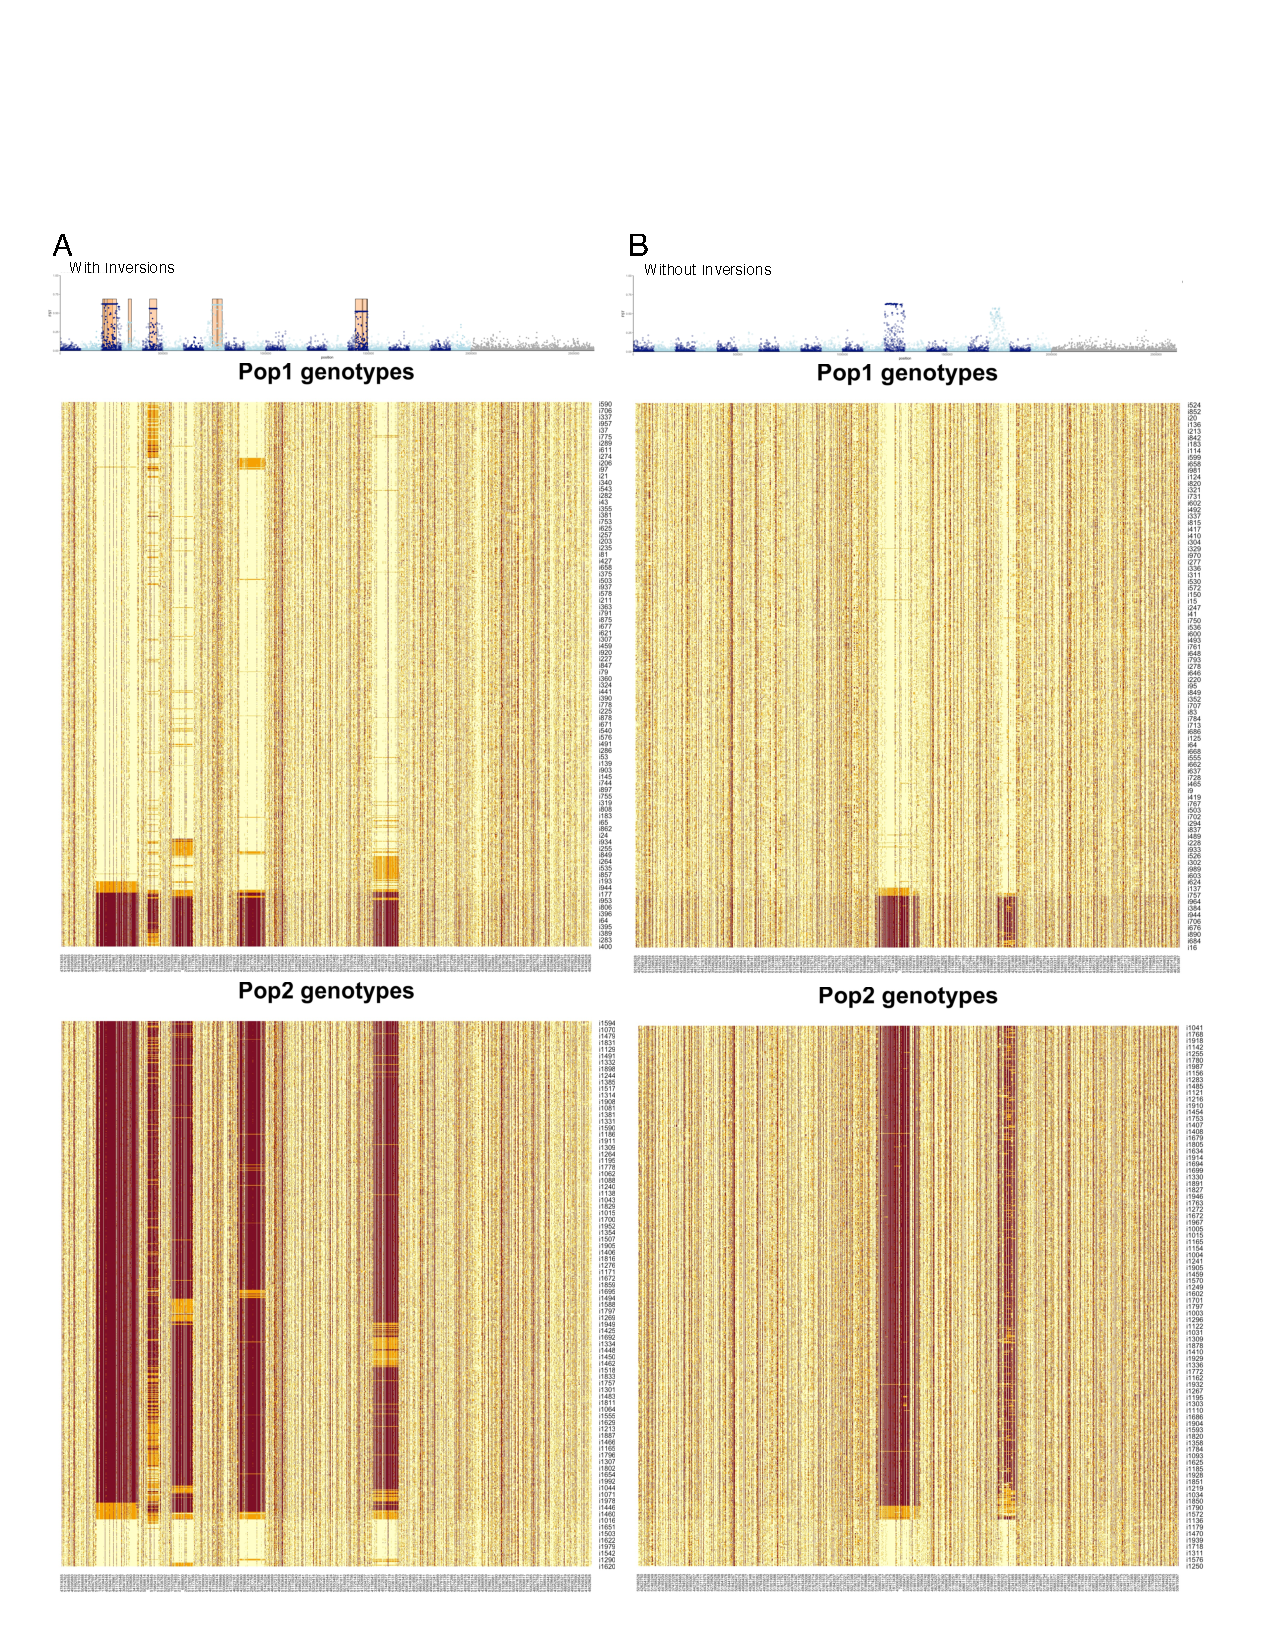
\includegraphics[width = 4.5 in]{FigS2_Heatmaps.pdf}
	\end{center}
	\caption[Heatmaps of the genetic architecture of divergence]{Manhattan plots with F\textsubscript{ST} of all QTNs in the genome as a function of chromosome position for A ) simulation where inversions facilitated adaptation and B) the paired no inversion control on the top panel that evolved strong islands of divergence (mig = 0.25, strong selection, polygenic architecture). Corresponding heatmaps are plotted below each manhattan plot and are colored by the genotype at a given locus for each individual in population 1 (middle panel) and population 2 (bottom panel). Yellow bars in manhattan plots represent regions that have an inversion. Dark and light blue colors for QTNs are alternated for each chromosome with the final all neutrally evolving chromosome in grey. }
\end{figure}

\clearpage
\newpage


\begin{figure}[h]
	\begin{center}
		\includegraphics[width = 4.5 in]{./Supplementary/FigS4_selectSim.pdf}
	\end{center}
	\caption[Genome Scan Performance for Selection Simulations]{Average number of adaptive QTNs either called correctly as outliers (blue bars) or incorrectly called as nonoutliers (yellow bars) and average number of nonadaptive QTNs either called correctly as nonoutliers (navy bars) or incorrectly called as outliers (golden bars) for A) PCAdapt and B) OutFLANK. Results are plotted for an oligogenic architecture in the top row and polygenic architecture in the bottom row. PCAdapt showed a slight increase in the number of adaptive nonoutliers in selection simulations when the trait was polygenic (Fig S5A see adaptive inversion indicated by black arrow in example manhattan plot where PCAdapt shows no outliers called inside that region). Conversely, OutFLANK showed a slight increase in the number of nonadaptive outliers in selection simulations when gene flow between populations was low under a polygenic architecture (Fig S5B see inversion indicated by black arrow in example manhattan plot where OutFLANK shows outliers called inside a nonadaptive inversion region). }
\end{figure}

\clearpage
\newpage

\begin{figure}[h]
	\begin{center}
		\includegraphics[width = 6.5 in]{FigS5_manh_outliers.pdf}
	\end{center}
	\caption[Incorrect Outlier Examples]{Manhattan plots depicting either the FST of QTN loci (Top row across panels) or the empicial p-value for two different outlier detection methods, OutFLANK (middle row) and PCAdapt (bottom row), as a function of genomic position. Each point represents a QTN loci with alternating dark and light blue circles in the top panel representing each chromosome with loci under selection and light grey squares being the neutrally evolving chromosome. In the six outlier panels (middle and bottom rows), black filled in dots and red open circles represent nonoutlier and outlier loci, respectively. All gold bars represent inverted regions that are present in the simulation. Adaptive inversions are depicted in panel A with the black arrow identifying an inversion that was not identified as an outlier in PCAdapt. Panel B shows nonadaptive inversions with an arrow identifying an inversion that was called as an outlier in OutFLANK. Panel C shows inversions from the no-selection control simulation with an arrow identifying a nonadaptive inversion that was called as an outlier in PCAdapt.}
\end{figure}

\clearpage
\newpage

\begin{figure}[h]
	\begin{center}
		\includegraphics[width = 4.5 in]{./Supplementary/FigS6_noSelect.pdf}
	\end{center}
	\caption[Genome Scan Performance for No-Selection Simulations]{Average number of nonadaptive QTNs either incorrectly called as outliers (blue bars) or correctly called as nonoutliers (yellow bars) for A) PCAdapt and B) OutFLANK. Results are plotted for an oligogenic architecture in the top row and polygenic architecture in the bottom row. PCAdapt showed a slight increase in false positives in control no-selection simulations when the trait was polygenic and migration rate was high (Fig S5C see inversion indicated by black arrow in example manhattan plot where PCAdapt shows outliers called inside a nonadaptive inversion region from a no-selection simulation). Error bars represent a single standard deviation among five replicate simulations.}
\end{figure}

\clearpage
\newpage



\end{document}



